% the-field-not-the-window__2026-09-03.tex — compiled from the slipcase; see the-field-not-the-window__SOURCE_MAP.txt
% Package: slipcase__ldraw-assembly-field__2026-09-03.zip · Return path: 000__RETURN_PATH.txt
\documentclass[11pt,a4paper]{article}
\usepackage[utf8]{inputenc}\usepackage[T1]{fontenc}\usepackage{graphicx}\usepackage{booktabs}\usepackage[margin=22mm]{geometry}\usepackage{hyperref}
\title{The Field, Not the Window\\\large Open ports, solicitation, and the attention tax of LDraw as a language of assembly}
\author{W. Hartsoe (whartsoe3@gatech.edu), Georgia Institute of Technology}
\date{Working Paper $\cdot$ AI-augmented research process $\cdot$ Evidence, prompts, and making history preserved\\2026-09-03}
\begin{document}
\maketitle
\begin{abstract}Language models that assemble LEGO models in the LDraw format fail in characteristic ways: pieces that hover, pieces that interpenetrate, pieces placed off the stud lattice. The usual remedy is to put more of the model into the context window. This paper argues that the remedy is aimed at the wrong object. LDraw records where a piece is, not what it can connect to, so a model reading LDraw must recompute connectability from coordinates before it can act; that recomputation, not token count, is the attention tax. Following the distinction between a landscape of affordances and the field of affordances that currently solicit action, the paper proposes that the representation an assembling model should see is the small, changing field of open ports of the half-built object, and that the model should answer with a relation to a port rather than a coordinate. A cheap instrument makes the field measurable: a stud faces air when the point just above it lies inside no other piece. Sixteen real kits keep between 11\% and 43\% of their structural studs open; of six generated builds in the same repository, 2 sit above that band and the rest inside it. A pass that closes every open stud drives 5 of 6 builds below the band and a twelve-axis critic calibrated on the kits barely registers the change, while a pass restricted to ragged surfaces moves one build from 5 wins / 7 losses to 6 wins / 6 losses. Applied to the kits themselves, the closing pass tiles over surfaces they leave open on purpose. The evidence therefore supports the field and refutes its naive reading: what must be routed to attention is solicitation, weighted by raggedness, reachability and intent, not the set of open ports. The paper closes with the seven prompt seeds this implies and with what remains unmeasured.\end{abstract}
\noindent\textbf{Keywords:} LDraw, assembly, affordances, attention, language models, stigmergy, LEGO, proprioception
\section*{1. Introduction}
A castle of six thousand pieces will not fit in the head of anything that has to place the next piece. This is as true of a person with a manual as of a language model with a context window, and the two cope in different ways. The person never holds the castle; they hold the piece in hand and a few places it might go. The language model, given the castle as LDraw text, is asked to hold all of it, and it reads coordinates. Each line of an LDraw file says which part sits at which position under which rotation \cite{ldrawformatspec}. Nothing in the line says whether the part is seated on studs, hovering a plate above them, or passing through a wall. Those facts are recoverable from the coordinates, but only by recomputing the geometry of every neighbour. That recomputation is the tax this paper is about.

The thesis is that the tax is representational rather than quantitative, and that it is paid whenever information which could stay implicit in the object is forced through a general-purpose description before action. The fix is not a larger window and not a shorter file. It is to show the model a different object: the field of open ports of the half-built model, ranked by how much each one currently solicits a piece, and to let the model answer with a relation to one of those ports. The argument borrows its central distinction from ecological psychology, where the landscape of affordances is what an environment offers in general and the field of relevant affordances is the small subset that stands out to a skilled agent in a concrete situation \cite{vandijk2017foregrounding}. The claim here is that an assembling model should be built to see the field.

The paper then does what the argument invites: it measures the field. A stud faces air when the point just above it lies inside no other piece. Counted across sixteen real kits and six generated builds in one repository, the number puts the kits in a band and the builds inside or above it, and a placement pass routed by that number changes the builds in a way a kit-calibrated critic almost cannot see. The naive version of the field, treated as a to-do list, makes the builds less like kits, not more. That result is the paper's stepping stone: the field is a field of solicitations, and solicitation has to be weighted by something the open-port count does not contain. The last section names the prompt seeds that follow and says where the evidence stops.

\section*{2. Where the argument comes from}
Three literatures meet here. The first is the ecological account of action, in which perception delivers possibilities for action rather than descriptions of the world, and skill consists in responding to the few possibilities that matter now \cite{vandijk2017foregrounding}. Cisek's affordance competition hypothesis gives the account a mechanism: the brain specifies several currently possible actions in parallel and lets them compete, with attention operating as an early selector among candidate actions rather than as a better reader of the scene \cite{cisek2007affordance}. Kirsh adds that agents arrange space so that the geometry performs some of the reasoning \cite{kirsh1995space}, and Brooks that a live world can answer questions a stored description would only approximate \cite{brooks1991intelligence}. These are arguments about biological and robotic agents. They transfer to an assembling language model because the model, too, has to choose among many possible next placements from a partial view.

The second literature is about coordination through the built object. Grassé's stigmergy, reviewed for construction by Smith and colleagues, describes builders whose next act is cued by the state of what has already been built rather than by messages \cite{smith2018architecture}; Werfel, Bar-Yam and Nagpal extend the idea so that construction blocks themselves carry machine-readable state \cite{werfel2005stigmergy}; Wilsson's beavers repair where the sound of running water recruits them \cite{wilsson1962beaver}. Control theory supplies the formal version: an expensive controller need not run on every tick if it runs whenever an error crosses a threshold \cite{tabuada2007event}, and an error should be weighted by how much the sensor reporting it can be trusted \cite{friston2011active}. Ashby's ultrastable system says when a deeper adaptation should be recruited at all: when an essential variable leaves its admissible region, not when the current step is merely hard \cite{ashby1960design}.

The third literature is the one the assembling model actually lives in. The LDraw file format is a recursive grammar: a type-1 line takes a reusable file, transforms it, and places an instance \cite{ldrawformatspec}. What it lacks is connectivity. Roland Melkert's shadow library for LDCad supplies snap metadata that the primary parts do not carry \cite{melkertldcadshadow}, and BrickNet builds from LDraw a connector graph and a build tree so that a generative model predicts relations rather than absolute poses \cite{kulits2026bricknet}. LegoGPT shows a generator that guesses, tests physics, and rolls back \cite{pun2025legogpt}; CADCodeVerify closes a loop of generate, render, interrogate and correct \cite{alrashedy2025cadcodeverify}; State-CAD keeps an authoritative structured state apart from the transcript \cite{lin2026statecad}. OmniCAD reports that frontier multimodal agents still fail on assemblies averaging about twelve parts \cite{wang2026omnicad}, which is the scale at which the argument of this paper begins to matter.

\section*{3. The argument}
\paragraph{3.1 LDraw knows where a piece is, not what it can connect to.} The point deserves to be stated plainly because it is easy to mistake for a complaint about verbosity. An LDraw placement is complete as geometry and silent as assembly: it can describe a brick that floats, a brick inside another brick, or a brick that could never have been inserted, using exactly the syntax it uses for a seated one \cite{ldrawformatspec}. Community tooling knows this, which is why connection data lives in a separate shadow library \cite{melkertldcadshadow} and why BrickNet had to reconstruct a connector graph before a model could be trained to build \cite{kulits2026bricknet}. A language model reading raw LDraw is therefore asked to do at inference what BrickNet did at preprocessing: infer relations from positions. Every hovering brick in a generated model is that inference failing silently.

\paragraph{3.2 The minimal representation for the next placement is the field of open ports.} If the model is not to hold the castle, what should it hold? The ecological answer is: what currently solicits action. For a stud-and-tube system this has an unusually literal form. Each piece exposes ports; a port is open when nothing occupies it; the set of open ports on the half-built model, together with the piece in hand, is the complete set of currently possible seated placements. This set is small relative to the model, it changes with every placement, and it is exactly what the human builder attends to when they look for where the next brick goes. Cisek's framing is the useful one: rather than represent the scene and then derive actions, derive the candidate actions directly from local geometry and let them compete \cite{cisek2007affordance}. Deictic roles then do the rest of the work: the open stud beside the last window is a better name than instance 5291 for the purposes of the next move, as Agre argued for everyday activity \cite{agre1988dynamic} and Pook and Ballard for teleassisted manipulation \cite{pook1996deictic}.

\paragraph{3.3 A field is not a to-do list.} Here the argument has to be careful, and the evidence in the next section shows why. An open port is a possibility, not an instruction. Real models leave surfaces open on purpose: a baseplate is a floor, a roof of studs is a roof, an open cavity is where the stair will go. A builder that treats every open port as a task to close will fill the cavity and make the stair impossible. This is the reward-shaping trap in its physical form: a local signal that looks like progress teaches a policy that changes which completions are reachable \cite{ng1999policy}. The field must therefore carry solicitation, not just openness. The candidates for what weights a port are the ones the stigmergy literature already names: raggedness (a surface partly covered solicits completion), adjacency to the working front (the beaver hears the leak, not the whole dam \cite{wilsson1962beaver}), the trust one has in the validator that reported the port \cite{friston2011active}, and the intent of the current sub-assembly.

\paragraph{3.4 Route the reasoner by the residual.} If the field is what the model sees, the residual is what it hears back. A refused placement should say what was placed, what was wanted, and what it cost in clashes, floats and open ports, because the useful part of a correction is the difference it points to; scalar reward teaches preference without vocabulary \cite{lightman2023verify,shinn2023reflexion}. And the expensive reasoner should be scheduled by that residual rather than by the clock: most placements in a castle are quiet repetitions, and event-triggered control says the controller runs when an error crosses a threshold, not on every step \cite{tabuada2007event}. Cook Ding's knife changes regime at the complicated joint and nowhere else \cite{zhuangziinner}. Put together, the four claims describe a builder whose prompt is not a sentence but the current field plus the last residual, and whose attention is spent where the object is ragged.

\section*{4. Evidence}
\paragraph{4.1 An instrument for the field.} To test whether the field is measurable at all, the compiler of this package wrote a probe over the repository's own catalogue (bounding boxes for 16,910 buildable parts) and port index (44,329 studs and tubes over 7,831 parts). A stud faces air when the point two LDraw units above its base, along the stud's own axis, lies inside no other placement's bounding box. Structural studs exclude baseplates and the ground level, which are open by design. The share of structural studs facing air is the shadow number. It is an approximation: the bounding box of a slope or an arch covers the air above its face, so coverage is an upper bound for such parts; the probe uses studs only and never tests whether a tube actually grips. Every number below was counted by that script and re-counted from the emitted files.

\paragraph{4.2 The kit band.} Sixteen real kits with pieces (the seventeenth is a single window brick) keep between 0.112 and 0.431 of their structural studs open, median 0.228. The two largest, the UCS AT-ST and the X-wing, sit at 0.112 and 0.368. The island hopper, which the repository uses as its default bar, is at 0.391, high because its hull is a plate field. Kits, in other words, are not closed objects; they are objects whose openness is placed.

\begin{table}[h]\centering\footnotesize\begin{tabular}{lrrrrr}\toprule kit & pieces & structural studs & open & share & open/piece\\\midrule
10174-imperial-atst-ucs & 1060 & 4842 & 540 & 0.112 & 0.584\\
1621-lunar-mpv & 104 & 293 & 59 & 0.201 & 0.694\\
30023-lighthouse & 25 & 114 & 19 & 0.167 & 0.792\\
30051-xwing-mini & 61 & 85 & 16 & 0.188 & 0.314\\
30054-atst-mini & 47 & 78 & 24 & 0.308 & 0.649\\
4489-atat-mini & 82 & 214 & 63 & 0.294 & 0.900\\
4494-imperial-shuttle-mini & 84 & 199 & 45 & 0.226 & 0.672\\
4838-mini-vehicles & 79 & 213 & 64 & 0.300 & 0.853\\
4915-mini-construction & 67 & 142 & 24 & 0.169 & 0.429\\
4918-mini-flyers & 75 & 193 & 44 & 0.228 & 0.710\\
5935-island-hopper & 203 & 875 & 342 & 0.391 & 2.060\\
6965-tie-interceptor & 32 & 51 & 22 & 0.431 & 0.957\\
6966-jedi-starfighter-mini & 39 & 86 & 17 & 0.198 & 0.607\\
7140-xwing-fighter & 287 & 1312 & 483 & 0.368 & 2.047\\
889-radar-truck & 35 & 87 & 14 & 0.161 & 0.467\\
car & 61 & 130 & 36 & 0.277 & 0.735\\\bottomrule\end{tabular}\caption{Structural studs facing air in the sixteen kits with pieces (measure-field.js; \_RESOURCES/field-results.json).}\end{table}
\paragraph{4.3 The builds, before and after the field.} Six generated builds from the same repository were measured, then run through two versions of a field-routed closing pass. The close-all pass tiles every open structural stud it can reach without clashing (2$\times$2, 1$\times$2 and 1$\times$1 tiles in the host's colour). The ragged pass tiles only studs on pieces whose top is already partly covered. Before the pass, 4 of 6 builds are inside the kit band; the castle is, at 0.227, and the crewed expedition ships are not, at 0.553 for the Beagle. The close-all pass takes 5 of 6 builds below the band (the sixth, the finch cactus, lands on its floor): the castle goes from 225 open studs to 12, adding 80 tiles. The ragged pass leaves 6 of 6 inside the band.

\begin{table}[h]\centering\footnotesize\begin{tabular}{lrrrrrl}\toprule build & pieces & before & close-all & ragged & tiles A/B & verdict W/L\\\midrule
card-castle & 182 & 0.227 & 0.019 & 0.148 & 80 / 27 & 4/8 $\rightarrow$ 4/8 $\rightarrow$ 4/8\\
card-fallingwater & 93 & 0.419 & 0.000 & 0.419 & 274 / 0 & 1/11 $\rightarrow$ 3/9 $\rightarrow$ 1/11\\
gauntlet-shore-station & 208 & 0.426 & 0.088 & 0.346 & 151 / 31 & 5/7 $\rightarrow$ 4/8 $\rightarrow$ 6/6\\
hms-beagle & 648 & 0.553 & 0.046 & 0.382 & 616 / 203 & 1/11 $\rightarrow$ 1/11 $\rightarrow$ 1/11\\
finch-cactus & 78 & 0.541 & 0.126 & 0.186 & 50 / 42 & 1/11 $\rightarrow$ 2/10 $\rightarrow$ 2/10\\
medusa-scriptorium & 1672 & 0.367 & 0.019 & 0.149 & 1493 / 972 & 1/11 $\rightarrow$ 1/11 $\rightarrow$ 1/11\\\bottomrule\end{tabular}\caption{Six repository builds before and after the two closing passes; kit band 0.112--0.431.}\end{table}
\begin{figure}[h]\centering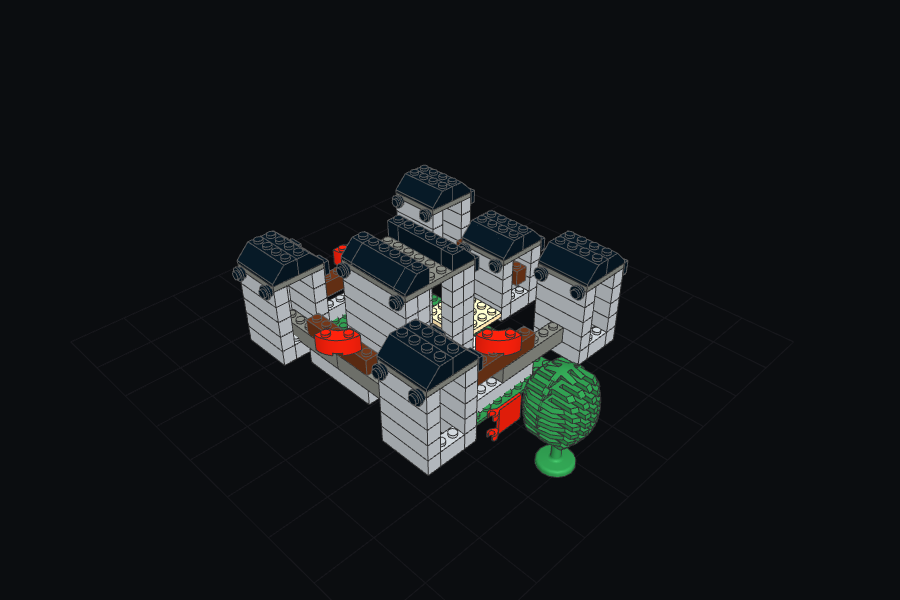
\includegraphics[width=.32\textwidth]{_RESOURCES/render__card-castle__before.png}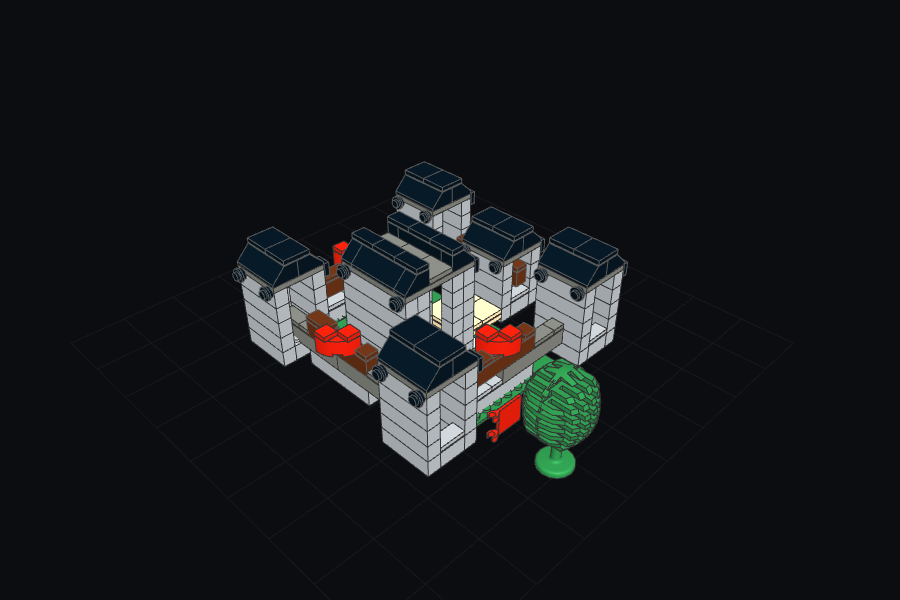
\includegraphics[width=.32\textwidth]{_RESOURCES/render__card-castle__A-close-all.png}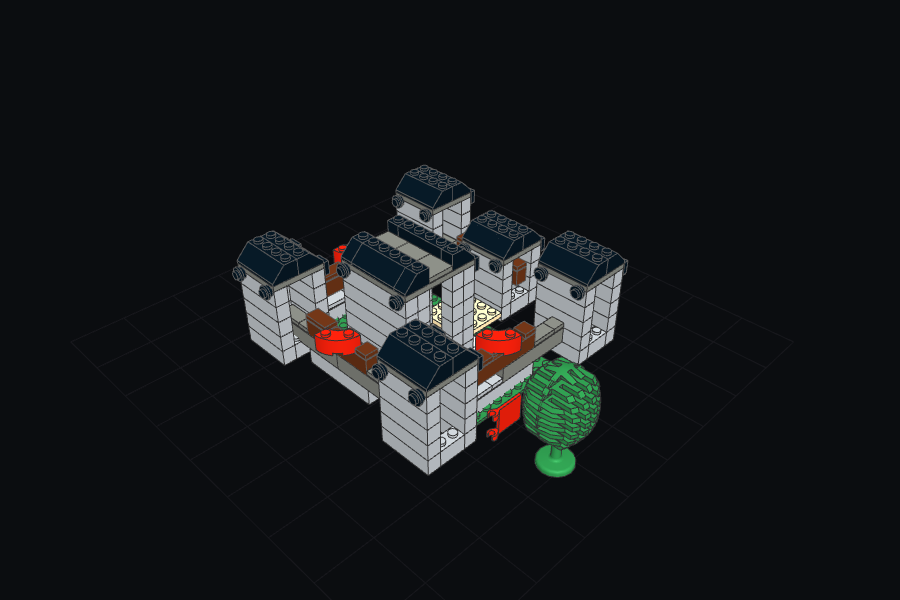
\includegraphics[width=.32\textwidth]{_RESOURCES/render__card-castle__B-ragged.png}\caption{The castle card build before the pass, after close-all, and after the ragged pass. Same camera, same viewer.}\end{figure}
\paragraph{4.4 What the critic saw.} The repository judges builds against a kit on twelve axes, blind, per axis and never summed, with ties going to the kit. On the castle the verdict is 4 wins / 8 losses before the pass and 4 wins / 8 losses after close-all: the same count, with colour flipping to a win and lattice flipping to a loss. On the shore station the ragged pass moves the verdict from 5 wins / 7 losses to 6 wins / 6 losses; on the fallingwater card the close-all pass moves it from 1 wins / 11 losses to 3 wins / 9 losses. A change that removes 213 open studs from a 182-piece model is nearly invisible to a critic that measures vocabulary, colour, rotation, symmetry and density. The critic has no proprioceptive axis.

\paragraph{4.5 The control.} Applied to two real kits, the close-all pass adds 103 tiles to the island hopper and 143 to the X-wing, tiling over hull plates and wing surfaces that the designers left open, and drives their open-stud ratio from 1.773 to 0.183 per piece. The pass is wrong on the kits, and it is wrong in the way section 3.3 predicted: it reads possibility as obligation.

\section*{5. Discussion}
The evidence supports the field and refutes the to-do list, and the refutation is the more useful half. The naive field is the very error the affordance literature warns against: mistaking the landscape for the field. What the kits show is that openness is placed. A surface that is entirely open is a design decision; a surface that is half covered is a solicitation. The ragged rule is a crude approximation of that difference and already behaves better on the kits than the close-all rule, which is what one would expect if the weight on a port should come from the state of its neighbourhood rather than from the port itself. Werfel's extended stigmergy suggests the next step: let sub-assemblies declare their open interfaces and their do-not-close cavities, so that the field is partly authored by the object \cite{werfel2005stigmergy}.

The second finding is about the critic. A twelve-axis judge calibrated on kits is nearly blind to whether pieces are seated. That is not a flaw in those axes; it is a gap. The bar for legibility should carry at least one proprioceptive axis, and the shadow number is a candidate: the share of structural studs facing air, judged like the others, in a band, blind, with ties to the kit. An axis of that kind is also the first one that a placement policy routed by the field would move directly, which makes it the right place to test the prompt seeds that follow from the argument.

The third implication is for the prompt. If the field is what the model should see and the residual is what it should hear, then the prompt at castle scale is not a sentence and not a serialised model. It is a small packet: the ranked open ports, the piece in hand as a body line, the card's intent for this region, and the last residual. Seven seed prompts built on that packet accompany this paper; only the first has been run, in its cheapest form, and its numbers are the ones above. The others are stated as hypotheses with their measures and mutation operators, so that they can be tested and evolved rather than believed.

\section*{6. Limitations and unresolved territory}
The probe is geometric, not mechanical. It says a stud is covered when something sits above it; it does not say that a tube grips it, and it cannot see hinges, clips, pins or bars, whose ports are absent from the index. A proper clutch test (a tube centre within the stud's ring, coplanar) has not been written. Bounding boxes overstate coverage under slopes and arches. Seventeen kits from one loader example are a small and biased bar. No language model was in the loop: the pass is a fixed rule, so the evidence bears on the representation, not yet on whether a model can use it. The earlier body-line and joints computation from the originating session is not preserved here and is treated as unverified.

The card field this paper draws on is itself incomplete. Sixteen addresses it cites, among them the prompt-praxis cards that ground the language-game argument, are ghosts: named, linked to, and not present in the package. They are held open as questions. The assembly-theory cards in the field (whether LDraw's reuse is compression or construction, what counts as an elementary part, whether a threshold like fifteen means anything for bricks) are adjacent to this argument and were deliberately not pulled into it; the evidence here does not reach them.

\section*{7. Conclusion}
A model that assembles in LDraw pays a tax every time it recomputes from coordinates what the object already knows about itself. The tax is not paid in tokens; it is paid in floating and interpenetrating pieces. The way to stop paying it is to show the model the object's field of open ports and let it answer with a relation. Measured across real kits and generated builds, the field is real, cheap to compute, and it tells a placed openness from an accidental one. Treated as a list of things to close, it makes builds worse and would ruin the kits. Treated as a field of solicitations, weighted by how ragged and how reachable each port is, it is the smallest representation from which competent next action follows. That is the wager. The instrument, the numbers, the cards, and the seeds to test the wager are in the package this paper ships with.

\begin{thebibliography}{99}
\bibitem{ldrawformatspec} LDraw.org Standards Board. (2012). LDraw File Format Specification. LDraw.org. Revision 1.0.2.
\bibitem{vandijk2017foregrounding} Ludger van Dijk, Erik Rietveld et al. (2017). Foregrounding Sociomaterial Practice in Our Understanding of Affordances: The Skilled Intentionality Framework. Frontiers in Psychology. vol. 7. pp. 1969.
\bibitem{cisek2007affordance} Paul Cisek. (2007). Cortical Mechanisms of Action Selection: The Affordance Competition Hypothesis. Philosophical Transactions of the Royal Society B. vol. 362. pp. 1585--1599.
\bibitem{kirsh1995space} David Kirsh. (1995). The Intelligent Use of Space. Artificial Intelligence. vol. 73. pp. 31--68.
\bibitem{brooks1991intelligence} Rodney A. Brooks. (1991). Intelligence without Representation. Artificial Intelligence. vol. 47. pp. 139--159.
\bibitem{smith2018architecture} (2018). Architecture, Space and Information in Constructions Built by Humans and Social Insects: A Conceptual Review. Philosophical Transactions of the Royal Society B.
\bibitem{werfel2005stigmergy} Justin Werfel, Yaneer Bar-Yam, Radhika Nagpal. (2005). Construction by Robot Swarms Using Extended Stigmergy. MIT Computer Science and Artificial Intelligence Laboratory.
\bibitem{wilsson1962beaver} Lars Wilsson. (1962). Observations on the Dambuilding Behavior of the Beaver (Castor Fiber L.). National Technical Information Service.
\bibitem{tabuada2007event} Paulo Tabuada. (2007). Event-Triggered Real-Time Scheduling of Stabilizing Control Tasks. IEEE Transactions on Automatic Control. vol. 52. pp. 1680--1685.
\bibitem{friston2011active} (2011). Active Inference, Attention, and Motor Preparation. Frontiers in Psychology. vol. 2. pp. 218.
\bibitem{ashby1960design} W. Ross Ashby. (1960). Design for a Brain: The Origin of Adaptive Behaviour. Chapman and Hall.
\bibitem{melkertldcadshadow} Roland Melkert. LDCad Shadow Library. LDraw snapping and mirroring metadata.
\bibitem{kulits2026bricknet} Peter Kulits, Cordelia Schmid. (2026). BrickNet: Graph-Backed Generative Brick Assembly. Proceedings of the IEEE/CVF Conference on Computer Vision and Pattern Recognition. pp. 39252--39261.
\bibitem{pun2025legogpt} Ava Pun, Kangle Deng, Ruixuan Liu, Deva Ramanan, Changliu Liu, Jun-Yan Zhu. (2025). Generating Physically Stable and Buildable LEGO Designs from Text. Proceedings of the IEEE/CVF International Conference on Computer Vision.
\bibitem{alrashedy2025cadcodeverify} Kamel Alrashedy, Pradyumna Tambwekar, Zulfiqar Haider Zaidi, Megan Langwasser, Wei Xu, Matthew Gombolay. (2025). Generating CAD Code with Vision-Language Models for 3D Designs. International Conference on Learning Representations.
\bibitem{lin2026statecad} Dawei Lin, Yuanning Liu. (2026). State-CAD: Precise and Iterative CAD Modeling with Structured State Representation and Reinforcement Learning. Computer-Aided Design. vol. 199. pp. 104128.
\bibitem{wang2026omnicad} Mingjia Wang et al. (2026). OmniCAD: A Large-Scale Benchmark for 3D Spatial Reasoning in Robotics Assemblies. arXiv preprint arXiv:2608.22637.
\bibitem{agre1988dynamic} Philip E. Agre. (1988). The Dynamic Structure of Everyday Life.
\bibitem{pook1996deictic} Polly K. Pook, Dana H. Ballard. (1996). Deictic Human/Robot Interaction. Robotics and Autonomous Systems. vol. 18. pp. 259--269.
\bibitem{ng1999policy} Andrew Y. Ng, Daishi Harada, Stuart Russell. (1999). Policy Invariance Under Reward Transformations: Theory and Application to Reward Shaping. Proceedings of the Sixteenth International Conference on Machine Learning. pp. 278--287.
\bibitem{lightman2023verify} Hunter Lightman, Vineet Kosaraju, Yura Burda, Harri Edwards, Bowen Baker, Teddy Lee, Jan Leike, John Schulman, Ilya Sutskever, Karl Cobbe. (2023). Let's Verify Step by Step. arXiv preprint arXiv:2305.20050.
\bibitem{shinn2023reflexion} Noah Shinn, Federico Cassano, Edward Berman, Ashwin Gopinath, Karthik Narasimhan, Shunyu Yao. (2023). Reflexion: Language Agents with Verbal Reinforcement Learning. arXiv preprint arXiv:2303.11366.
\bibitem{zhuangziinner} Zhuangzi. Inner Chapters: Nourishing the Lord of Life. Cook Ding passage; received pre-Qin text.
\end{thebibliography}
\section*{Appendix A --- Assembly instrument}
The exact prompt that assembled this publication is preserved verbatim as \_PROMPTS/00\_\_ASSEMBLY-PROMPT\_\_SLIPCASE-POML.txt in the package (18671 characters, sha256 7f5a482718cb12b6b1fcc36878653e7dcec563dcf1de407f524c615c408ada75), inside index.html, and as \_RESOURCES/poml\_\_SLIPCASE-PORTABLE-RESEARCH-FIELD\_\_15.55-AM.txt. It is too large to reproduce here; it is a POML document (version 15.55-AM) whose meta, role, stance, model, laws, cards, graph, publication, index, reader, bibliography, resources, paper, provenance, mark, return\_path, verification, process, adapt, design and final\_test sections define this package. The request line that preceded the zettel batches is preserved as \_PROMPTS/00\_\_REQUEST-LINE.txt.
\section*{Appendix B --- Making history}
PROVIDED: 87 zettels and one POML assembly prompt, pasted by the researcher into one session on 2026-09-03; the repository tractor-dce-gyo (catalogue, port index, 17 kits, 11 builds, the twelve-axis critic).

PRESERVED: every payload byte-exact as a root .txt card and \_MD mirror; the POML verbatim; the raw paste under \_RESOURCES/.

RETRIEVED: nothing from the network. All DOI/URL receipts are LINK\_ONLY.

DERIVED: the open-stud probe and closing passes (measure-field.js), the renders, the tables in Sections 4.2--4.5, the graph, the MOCs and arrangements, and this paper's connective prose. The paper was written by the compiling model; the researcher had not reviewed it at packaging time.

VERIFIED: every number in Section 4 was counted by the script and re-counted from the emitted MPD files; citekeys used in the paper were checked against the compiled bibliography (see SOURCE\_MAP).

UNVERIFIED: the body-line/joints computation mentioned in Section 6 (not preserved); the accuracy of AABB coverage under slopes; any human review of the argument.
\section*{Appendix C --- Replication path}
Open index.html from the package by itself: it carries every payload, filename and hash, the bibliography, the resources registry with the bodies of text resources, the exact assembly prompt, the graph, ghosts and backlinks, the MOCs, this paper, its source map, the making history and the rebuild instructions.

To verify a card: compare the SHA-256 of its root .txt file with ZETTELS.json. To rebuild the card box from the deck alone: python3 \_SLIPCASE/rebuild.py ZETTELS.jsonl <out-dir> regenerates every root card and \_MD mirror and checks each hash; the compiler ran that test before packaging (result in \_SLIPCASE/VERIFICATION.txt).

To reproduce the numbers: with the repository checked out, run node slipcase-build/measure-field.js (needs nabugo-parts.json, nabugo-ports.json, nabugo-kits.js, nabugo-gauntlet.js, kits/, builds/); it writes field-results.json. Renders need Chromium and the local kits.html viewer (render-field.js). The paper is regenerated by compile.py; its PDF was printed from the HTML twin with Chromium because no TeX installation was available; the .tex is provided for a TeX compile elsewhere.
\vfill\begin{flushright}\footnotesize Working Paper $\cdot$ AI-augmented research process $\cdot$ Evidence, prompts, and making history preserved. 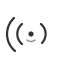
\includegraphics[height=14pt]{MARK.svg}\end{flushright}
\end{document}
